\chapter{Fundamentals of EPR}

In this chapter, the phenomenon of electron paramagnetic resonance is briefly described with details that are required to interpret the spectra of a charging electrochemical cell containing nitroxide radicals attached to a conjugated polymer backbone. After the introduction of the spin Hamiltonian, an experimental procedure to observe the corresponding spin transitions with continuous microwaves is described. The characteristic spectra of nitroxide radicals in various environments are described. Finally, the fundamentals and the experimental techniques of the pulsed EPR are introduced.

\subsection{The Spin Hamiltonian}
\label{sec:spin}
\paragraph*{Electron Spin}
In the Poincaré group of special relativity~\cite{poincare_1905}, when rotations are considered together with the relativistic boosts~\cite{einstein_s_rel}, there emerges an additional quantity that is associated with rotation and is preserved together with the orbital angular momentum, yet this quantity is retained for point objects - it is called spin~\cite{kuprov_2023}. Spin is quantized~\cite{SternGerlach1922}; it can take values in integer- or half-integer multiples of the Planck's quantum of action $\hbar$ up to a certain magnitude $S$. The electron, as a fundamental particle and a fermion, bears a half-integer spin with a magnitude of $S=1/2$~\cite{SternGerlach1922,Sakurai}. 

\par
An isolated electron has two degenerate spin states - spin-up $\vert{\uparrow}\rangle$ and spin-down $\vert{\downarrow}\rangle$ - that are eigenfunctions of the square of the spin operator $\hat{s}^2$ with the same (degenerate) eigenvalue $\hat{s}^2\vert{\uparrow}\rangle=\hat{s}^2\vert{\downarrow}\rangle=\frac{3}{4}\hbar^2$. The states $\vert{\uparrow}\rangle$ and $\vert{\downarrow}\rangle$ are also eigenfunctions of the $z$ component of the spin operator, but correspond to different (non-degenerate) eigenvalues $m_s=\pm\hbar/2$~\cite{Sakurai}: 

\begin{equation}
\label{eq:sz_states}
\hat{s}_Z\vert{\uparrow}\rangle = +\frac{\hbar}{2}\vert{\uparrow\rangle}
\end{equation}
\begin{equation*}
\hat{s}_Z\vert{\downarrow\rangle}=-\frac{\hbar}{2}\vert{\downarrow\rangle}
\end{equation*}


\paragraph*{$\textbf{g}$ factor}

Spin combines with the charge of the electron to endow the electron with a magnetic moment $\mu_{spin} = \gamma S$, where $\gamma=\frac{g_e\mu_B}{\hbar}\approx 28$~GHz/T is the gyromagnetic ratio of the electron, $\mu_B=\hbar e/m_e$ is the Bohr magneton and $g_e \approx 2$ is the electron $g$ factor~\cite{Carrington_g_factor}. The $g$ factor connects the spin of a particle with a magnetic moment that the particle expresses through interactions with external fields~\cite{Schwinger1948}. The Dirac quantum theory of the electron predicts $g_e=2$~\cite{dirac1928}. However, up to date, $g_e = 2.00231930436256(35)$ has been measured to the unprecedented accuracy of 0.13~ppt~\cite{Fan2023_PRL}. This measurement lies at the frontier of modern particle physics and the accordance of the measured $g_e$ with the value obtained with quantum electrodynamics~\cite{Schwinger1948,Fan2023_PRL} is the triumph of the quantum field theory~\cite{Feynman_1949}. 
\par
Depending on the local environment of an electron, its $g$ factor can change from $g_e$ due to the spin-orbit coupling that changes the observed magnetic moment of the electron~\cite{Carrington_g_factor}. The magnetic moment of an electron can therefore be used as an extremely sensitive probe of the electron's local environment. The $g$ factor of an electron localized in a molecular orbital can be anisotropic, depending on the shape of the orbital. Anisotropic $g$ factor is represented by a $3\times3$ $\textbf{g}$ matrix that can almost always be diagonalized~\cite{Carrington_g_factor} by an appropriate rotation of the molecular coordinate system.



\paragraph*{Zeeman Splitting}

When an electron is placed in a static magnetic field $\vec{B_0}=B_0 \vec{e_z}$, its magnetic moment experiences a torque and precesses in the $xy$ plane about the field axis with the Larmor frequency $\omega_L = \gamma B_0$. The magnetic moment of the electron has two possible projections on the magnetic field axis, according to \ref{eq:sz_states}. The two corresponding eigenvalues $\pm\frac{\hbar}{2}$ define the energy difference between the states $\vert{\uparrow\rangle}$ and $\vert{\downarrow\rangle}$ when the spin couples to the external magnetic field, that is known as the Zeeman splitting. The energy difference between $\vert{\downarrow}\rangle$ and $\vert{\uparrow}\rangle$ in a magnetic field is the Zeeman energy. 

\par

The energy of an isolated electron placed in the external magnetic field $\vec{B_0}$ is the energy of the electron's magnetic moment in that field, that is given by the eigenvalue of the spin Zeeman Hamiltonian: $\hat{H}_{EZ} = \frac{\mu_B}{\hbar} \vec{B}_0g_e\vec{\hat{s}}$. In the laboratory frame of reference $\vec{B_0}\parallel\vec{e_z}$, $\left[\hat{H}_{EZ},\hat{s}_z\right]=0$, so $\hat{H}_{EZ}$ and $\hat{s}_Z$ share the two eigenfunctions $\vert{\uparrow\rangle}$ and $\vert{\downarrow\rangle}$. The energies of the corresponding states are $E_{EZ}^{\pm} = \pm \frac{1}{2}\mu_B g B_0$ (see Figure~\ref{fig:cwerp_free_electron}), and their difference is the Zeeman splitting:

\begin{equation}
%\label{eq:epr_resonance_condition}
\label{eq:electron_zeeman}
\Delta E_{EZ} = \mu_B g_e B_0
\end{equation}

The measurement of the magnetic moment of an electron can be done by measuring its Zeeman energy. The local molecular environment affects the electron's magnetic moment through spin-orbit coupling which can be seen as a deviation in the electron's $g$ factor~\cite{Carrington_g_factor}.



\paragraph*{Nuclear Spin and Nuclear Zeeman Splitting}
A proton has a half-integer spin $S=1/2$ that results in a magnetic moment $\mu_p = \mu_e\frac{m_e}{m_p}$, that is $\frac{m_p}{m_e}\approx1836$ times smaller than the electron's magnetic moment. A neutron bears no charge but also has a half-integer spin $S=1/2$. An atomic nucleus that consists of protons and neutrons has a magnetic moment which is a vector sum of the aligned spins of its protons and neutrons. The spin of a nucleus is defined by the arrangement of its nucleons and by the nuclear charge. A nitrogen nucleus has 7 protons and 7 neutrons that total in a nuclear spin $I=1$ which, with the g factor for the nitrogen nucleus $g_N$, results in the nuclear magnetic moment of $\mu_N=\mu_B\frac{m_e}{m_N}g_NI$ that splits each of the electron Zeeman level into three nuclear Zeeman energy sublevels corresponding to the three possible projections of the nuclear spin on the magnetic field axis, $m_I=-1,0,+1$, analogously to the electron with $m_S=1/2,-1/2$. The two splittings are shown in the energy diagram in Figure~\ref{fig:energy_diagram}. The nuclear Zeeman splitting is more than two orders of magnitude weaker than the electron Zeeman splitting because of the difference in the masses of the particles.

\paragraph*{Hyperfine Interaction}
The magnetic moments of an electron and a magnetic nucleus, such as nitrogen, couple in the hyperfine interaction: $H_{HF}=\vec{\hat{s}}\textbf{A}\vec{\hat{I}}=H_F+H_{DD}$ with the hyperfine coupling tensor $\textbf{A}$. The isotropic part $H_F=a_{iso}\vec{\hat{s}}\vec{\hat{I}}$, or the Fermi contact interaction, scales with the probability density of the electron at the position of the nucleus $a_{iso}=\frac{2}{3}\frac{\mu_0}{\hbar}g_e\mu_eg_n\mu_n\vert\psi(0)\vert^2$~\cite{Schweiger2001}. The anisotropic part $H_{DD}=\vec{\hat{s}}\textbf{T}\vec{\hat{I}}$ with the dipolar coupling tensor $\textbf{T}$ takes into account the anisotropic magnetic dipole coupling between the magnetic moments of the electron and the nucleus. $\textbf{T}$ depends on the shape of the electron orbital, its $3\times3$ Cartesian matrix representation depends on the molecular frame of reference and can be diagonalized by rotating the coordinate system. The matrix representation of the hyperfine coupling tensor $\textbf{A}$ can be written in as the sum of its isotropic and anisotropic parts: $\textbf{A}=a_{iso}\mathds{1}_3 + \textbf{T}$~\cite{Weil_Bolton}. In its diagonal matrix representation $\textbf{A}$ reduces to its three principal components $[A_{xx}, A_{yy}, A_{zz}]$. The values of $\textbf{A}$ are typically given in MHz.

\paragraph*{Exchange Interaction}
In a system of closely placed electrons, such as in a film of densely packed radicals, the electron orbitals may overlap significantly and the radicals may exchange electrons. The energy required to exchange the electrons is called the exchange coupling $H_{exch} = \vec{\hat{s_1}}\textbf{J}\vec{\hat{s_2}}$, that becomes considerably large at inter-spin distances below $r<1.5$~nm or with a large spin delocalisation~\cite{Schweiger2001_exch}. The positive $\textbf{J}$ corresponds to a weak coupling between $s_1$ and $s_2$ which leads to an antiferromagnetic or antiparallel alignment of spins with a total $S=0$, whereas the negative $\textbf{J}$ causes the strong inter-spin coupling which leads to a ferromagnetic alignment with $S=1$~\cite{Schweiger2001_exch}.\\

%\paragraph*{Magnetic Dipole-Dipole Interaction}
%The dipole-dipole interaction between the two neighboring electron spins contributes one more term to the spin Hamiltonian: $H_{dd} = \vec{\hat{S_1}}\textbf{D}\vec{\hat{S_2}}$ that depends on the distance between the spins. 

\paragraph*{Nuclear Quadrupole Moment}
The nitrogen nucleus has a spin greater than 1/2 which alters the charge distribution within the nucleus which gives rise to a non-vanishing nuclear electrical quadrupole moment $Q$~\cite{Schweiger2001}. The interaction between the asymmetrically distributed charge and the gradient of the electric field at the nucleus is given by the nuclear quadrupole Hamiltonian $H_{NQ}=\vec{\hat{I}}\textbf{P}\vec{\hat{I}}$ with the nuclear quadrupole tensor $\textbf{P}$ that describes the coupling of the nuclear quadrupole moment to the electric field gradient.

\paragraph*{The Spin Hamiltonian}
For the interactions considered in this thesis, the following Hamiltonian will be applied to describe the interactions of unpaired electron spins with their local environments, ranging by their magnitude:
\begin{equation}
H = H_{EZ} + H_{HF} + H_{J} + H_{NZ} + H_{NQ}
\end{equation}

The electron Zeeman term $H_{EZ}$ defines the requirements on the hardware and sets the range of the magnetic fields used in the spectroscopic experiments. The hyperfine interaction term $H_{HF}$ allows for reconstruction of the hyperfine coupling tensor from the recorded spectra which is used as a marker to identify the molecular structure and dynamics of the mobile molecular fragments that are released during the operation of an electrochemical cell. The exchange interaction term $H_{J}$ scales with the concentration of the electrons, so the information about $\textbf{J}$ can be used to characterize the packing of the molecular fragments in the electrode. The nuclear quadrupole interaction term may lead to spectral distortions in a highly charged cathode where electric fields may be sufficiently strong to introduce noticeable nuclear quadrupole couplings to the nitrogen nuclei.

\begin{figure}[h]
\center
	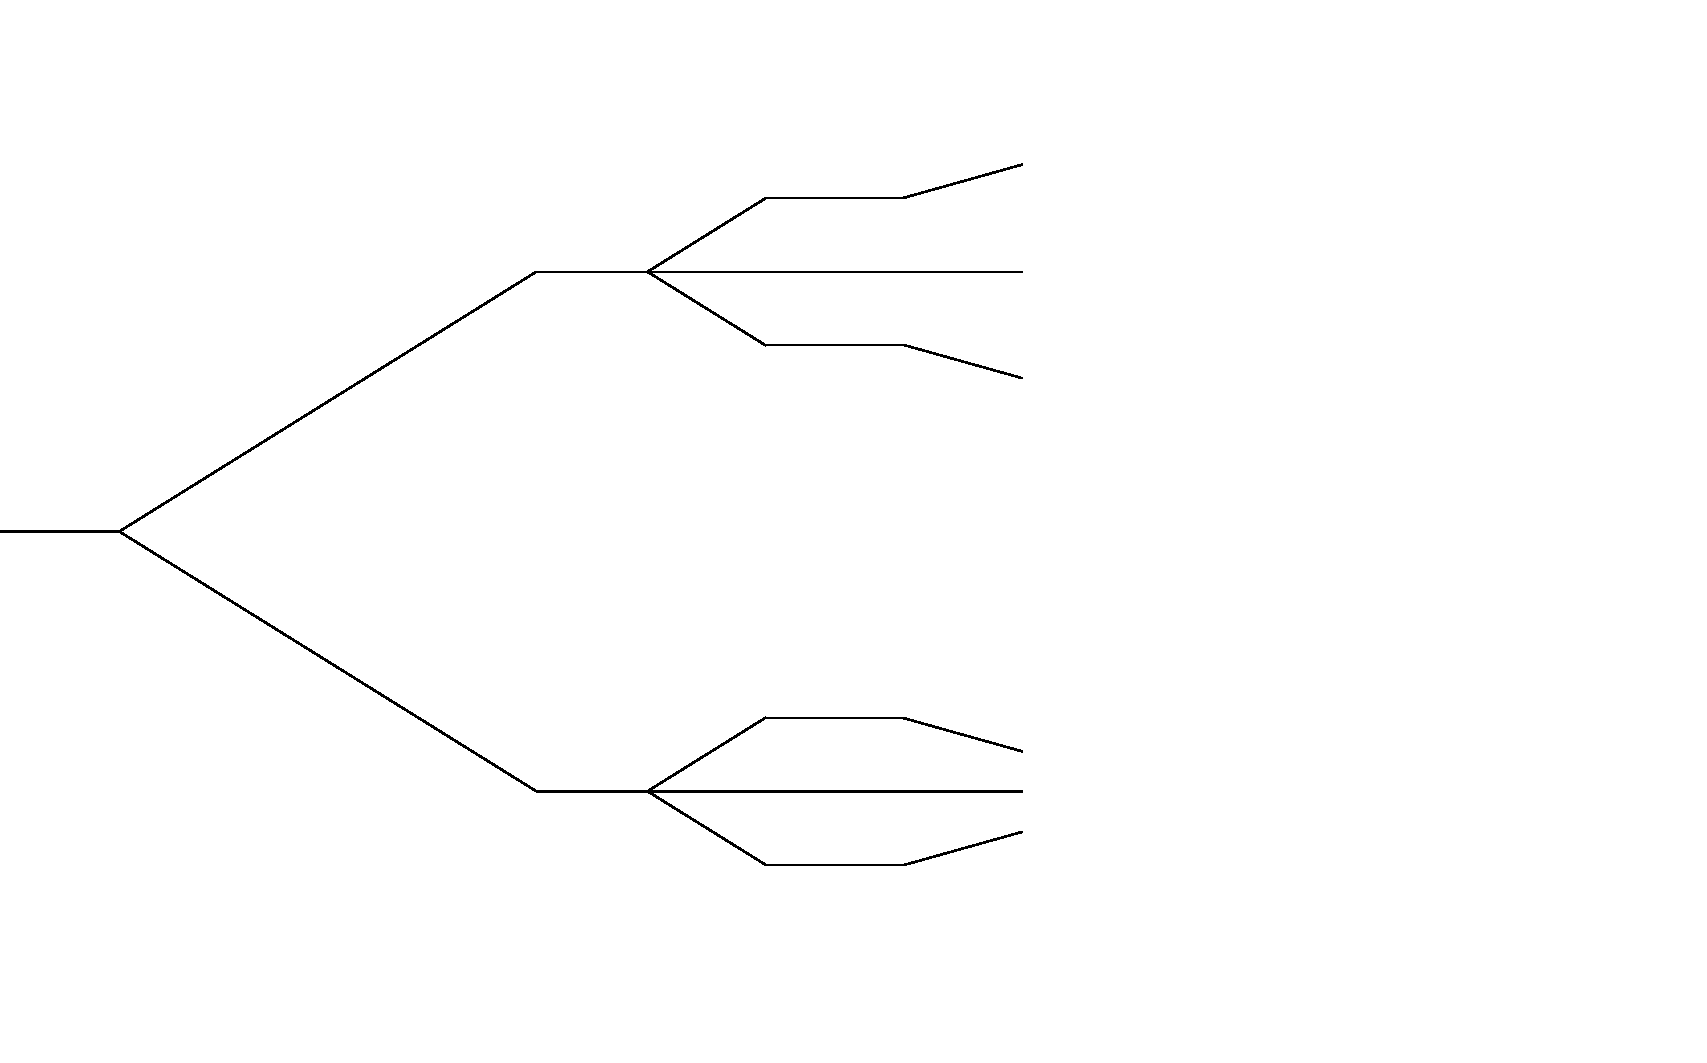
\includegraphics[width=1.0\textwidth]{./operando_epr/figures/energy_diagram.pdf}
	\caption{Energy diagram of the spin Hamiltonian showing the contributions of the individual terms.}
	\label{fig:energy_diagram}
\end{figure}



\subsection{cwEPR Instrumentation}
\label{subs:cwEPR_spectroscopy}
First observed in 1945~\cite{Zavoisky_1945_JP,zavoisky_1945,salikhov_2015}, the phenomenon of electron paramagnetic resonance had quickly become a tool for probing local molecular environments in species that contain unpaired electron spins. A free electron, that does not interact with its environment and has $g=g_e$, experiences a Zeeman splitting of $\Delta E = g \mu_B B_0$, that corresponds to the energy of a photon with a frequency of $\nu=\Delta E / h$. A microwave photon can drive a magnetic dipole transition between the Zeeman-split spin states - this is called electron paramagnetic resonance (EPR). An X band microwave photon (IEEE X band, $\nu=8-12$~GHz, $\lambda=2.5-3.8$~cm, Figure~\ref{fig:cwerp_free_electron}, left) can drive the magnetic dipole transition between $\vert{\uparrow\rangle}$ and $\vert{\downarrow\rangle}$ at $B_0\approx0.3$~T. In a continuous-wave electron paramagnetic resonance (cwEPR) experiment, the microwave frequency and power is kept constant while $B_0$ is scanned and the microwave absorption is observed. EPR happens around the $B_0$ values given by the spin resonance condition:

\begin{equation}
\label{eq:epr_resonance_condition}
\mu_B g_e B_0 = h\nu
\end{equation}

\begin{figure}[h]
\center
	\includegraphics[width=1.0\textwidth]{../scripts/plots/Free_Electron_EPRcombo.pdf}
	\caption{Left: Zeeman splitting for the energies of the two states of an isolated electron spin in a static magnetic field computed with EasySpin~\cite{Stoll2006}. Vertical line is the magnetic dipole transition driven by a $9.4$~GHz microwave photon. Right: Microwave absorption and its derivative as a function of the static magnetic field for an unpaired electron spin with a 5~mT Gaussian broadening.}
	\label{fig:cwerp_free_electron}
\end{figure}


\par
When $B_0$ reaches the value that satisfies Eq.~\ref{eq:epr_resonance_condition}, the sample starts absorbing microwaves. The absorbed microwave power recorded as a function of $B_0$ is the cwEPR spectrum (Figure~\ref{fig:cwerp_free_electron}, right, dashed). By construction, cwEPR spectrometers typically record the derivative of the microwave absorption vs. $B_0$ (Figure~\ref{fig:cwerp_free_electron}, right, solid). Advanced spin resonance techniques methods that involve coherent spin dynamics and pulsed microwave fields are discussed in Chapter~\ref{ch:pulsed_epr}.

\paragraph{cwEPR spectrometer}

A basic cwEPR spectrometer consists of a magnet, a microwave source, a resonator and a microwave detector. Figure~\ref{fig:cwerp_spectrometer} depicts those elements with more details, including the sample - an electrochemical cell that is placed inside the microwave resonator and its SoC controlled with an external potentiostat.

\begin{figure}[h]
\center
	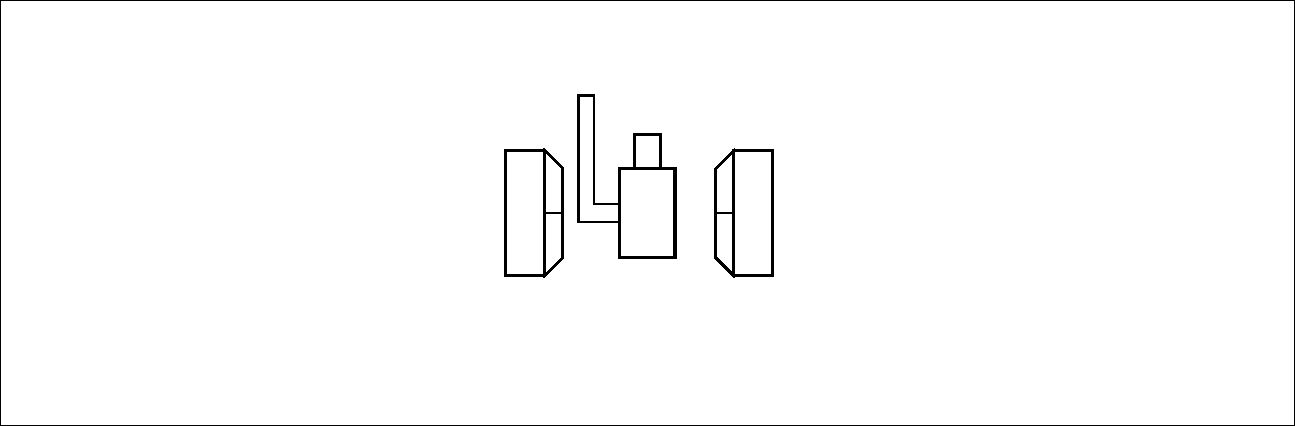
\includegraphics[width=0.9\textwidth]{./operando_epr/figures/cwEPR_spectrometer_diagram.pdf}
	\caption{Diagram of a cwEPR spectrometer}
	\label{fig:cwerp_spectrometer}
\end{figure}

\par
Continuous microwaves are generated with a klystron (MW source in Figure~\ref{fig:cwerp_spectrometer}) and directed towards the resonator (resonating cavity) through the signal arm that contains a variable attenuator and a circulator. The circulator directs the microwaves from the source to the cavity and passes the microwaves reflected from the cavity further to the microwave detector. The adjustable coupling iris between the circulator and the resonating cavity allows one to match the impedance of the cavity to the impedance of the signal arm so that minimal microwave power is reflected back from the cavity at a non-resonant field $B_0$. That impedance matching is called critical coupling. At the microwave detector, the microwaves reflected from the cavity are compensated by the microwaves with fixed microwave power and an adjustable phase, that pass through the reference arm. The signals from the two arms interfere destructively at the detector, so that there is no signal at the detector for non-resonant $B_0$.

\par
When the resonance condition (Eq.~\ref{eq:epr_resonance_condition}) is met, the incident microwaves are being absorbed by the sample and the resonator's $Q$ factor slightly changes. The change in the $Q$ factor decouples the resonator from the signal arm, that causes additional reflections in the signal arm. The microwaves in the signal arm that are not compensated by the reference arm become detected by the microwave detector - a biased semiconductor diode that has a linearly changing conductivity in the range corresponding to the incident microwave power. A phase sensitive detection with shallow modulation of $B_0$ increases the signal-to-noise ratio (SNR) and yields the derivative of the microwave absorption profile vs. $B_0$. The typically high $Q\gg1$ factor of the resonator further increases the SNR, as the decoupling of a resonator with higher $Q$ leads to a larger reflected microwave power.

\par
To ensure that only the magnetic component of the microwave is interacting with the sample, a standing microwave is formed in the resonating cavity. In the center of the cavity, the magnetic component of the microwave is maximized and the electric component is quenched. When a small sample is inserted in the center of the cavity, it is mostly the magnetic component of the microwave that is interacting with it. That allows one to drive magnetic dipole transitions without heating up the sample by the electric component. For larger samples as, for example, working electrochemical cells, the separation between the electric and magnetic microwave components does not hold within the full sample volume. Furthermore, the insertion of a cell containing metal electrodes and polar electrolyte into a resonator changes the distribution of the microwave field in it and lead to a non-resonant microwave absorption.


\paragraph{Line Broadening}
The lines in the EPR spectra have finite widths. The lines of the liquid samples are broadened mostly by the dynamic effects (relaxation, tumbling, chemical exchange), while the lines of solid state samples are broadened by static effects (orientational disorder, unresolved hyperfine splittings, distributions in $\textbf{g}$, $\textbf{A}$, and $\textbf{D}$ values)~\cite{Stoll2006}.\\

According to the stochastic, gaussian random modulation theory of exchange narrowing, the width of a strongly exchange narrowed EPR line (HWHM) is given by
\begin{equation}
\label{eq:exch_narrowing}
\Delta B_0 \approx\frac{10}{3}\left(\frac{H_p^2}{H_e}\right)
\end{equation}
and the resonance lineshape is lorentzian. $H_p$ is the mean square dipolar field and $H_e$ is an effective exchange field which is proportional to the mean exchange integral $J$~\cite{Oreilly_1971}


\section{Fundamentals of Pulsed EPR Spectroscopy
}
\subsection{Coherent Spin Motion under Pulsed Microwave Field}

The motion of the magnetization vector $\vec{M}(t,\vec{r})$ precessing in a static magnetic field $B_0$ is convenient to consider in the rotating frame of reference that has its $\vec{z^{\prime}}$ axis fixed to the magnetization vector ${\vec{z}}~^{\prime}\parallel\vec{M}$ so that the $x^{\prime} y^{\prime}$ plane rotates around $\vec{M}$ at the Larmor frequency $\omega_L=\gamma B_0$ when viewed from the laboratory frame $\vec{x},\vec{y},\vec{z}$, with $\gamma\approx2X$~MHz/T for the gyromagnetic ratio for electrons described in Section~\ref{sec:spin}. In the rotating frame, the macroscopic magnetization stays constant as long as the spin system interacts only with the static field $B_0$. When the spin system is excited with a linearly polarized microwave field $\vec{B_1}(t,\vec{r})\perp\vec{B_0}$, its evolution is described with the set of equations that is known as the Bloch equations (Eq.~\ref{eq:Bloch}). Let the microwave field of frequency $\omega_1$ and amplitude $B_1$ propagate along $\vec{z}$ and be polarized in the $xz$ plane: $\vec{B_1}(t,\vec{r})=B_1\vec{x}\cos\left(\omega_1t\right)$. The total magnetic field $\vec{B}=\vec{B_0}+\vec{B_1}$ causes a time-dependent torque on the $\vec{M}$ which leads to its precession - this time in the rotating frame of reference:

\subsection{Bloch Equations}
\begin{equation}
\label{eq:Bloch}
\frac{dM_x(t)}{dt} = \gamma\left(\vec{M}(t)\times\vec{B}(t)\right)_x - \frac{M_x(t)}{T_2}
\end{equation}
\begin{equation}
\label{eq:Bloch}
\frac{dM_y(t)}{dt} = \gamma\left(\vec{M}(t)\times\vec{B}(t)\right)_y - \frac{M_y(t)}{T_2}
\end{equation}
\begin{equation}
\label{eq:Bloch}
\frac{dM_z(t)}{dt} = \gamma\left(\vec{M}(t)\times\vec{B}(t)\right)_z - \frac{M_z(t)-M_0}{T_1}
\end{equation}



\subsection{Refocused Spin Echo}
\subsection{Spin Relaxation Times}
\subsection{Spin Packets}

\section{Pulsed EPR Instrumentation}

\begin{figure}[h]
\center
	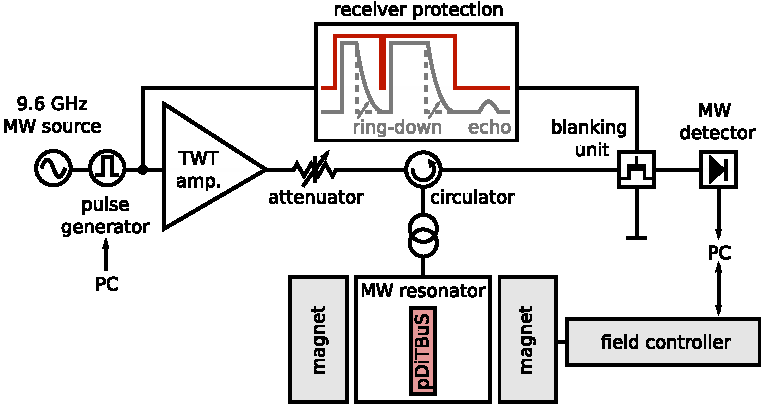
\includegraphics[width=1\textwidth]{./pulse/figures/pEPR_spectrometer_diagram.pdf}
	\caption{Diagram of a pulsed EPR spectrometer.}
	\label{fig:pepr_spectrometer_diagram}
\end{figure}

\subsection{Pulse Sequences and Measurement Techniques}
\subsubsection{The Refocused Spin Echo Sequence}
The Hahn Echo sequence consists of two pulses, the $\pi/2$ pulse and the $\pi$ pulse, separated in time by $\tau$: $\pi/2 - \tau - \pi - \tau - echo$. Initially, the macroscopic magnetization of the spin system is aligned along $\vec{B_0}$: $\vec{M}_0=M_Z~\vec{e_Z}$. The $\pi/2$ microwave pulse has such length $t_{\pi/2}$ and amplitude $B_1$ that, during the pulse, $\vec{M}$ nutates to the $xy$ plane, where it keeps precessing about $\vec{e_Z}$ after the end of the pulse. The difference in local environments for each individual spins in the spin packet, as well as the interactions between the spins, that make up $\vec{M}$, leads to slightly different precession frequencies $\omega_L^i$ of the spins. After some time $\tau$, the difference in the precession frequencies translates into the differences in phases so that the vector sum of the excited spins averages down to $\vec{0}$ for sufficiently long $\tau$. In other words, the excited spin packet dephases with time. The dephasing due to different local spin environments can be reversible if the deviations of the precession frequencies do not depend on time, as is the case for separated electrons in an inhomogeneous solid. In such case, a $\pi$ pulse can be applied to the spin system to flip every single spin in the dephased spin packet by 180$\deg$ in a plane containing $\vec{e}_Z$, so that the spins keep precessing in the $xy$ plane, but the direction of precession is inverted for them, leading to the effect that is opposite to the initial dephasing. So a $\tau$ after the $\pi$ pulse excites the spin packet, the accumulated phase differences become the smallest and the packet recovers its macroscopic magnetization $\vec{M}$ that oscillates in the $xy$ plane with $\langle\omega_L^i\rangle$ and can be detected. The recovered $\vec{M}$ at $t=\tau$ after the $\pi$ pulse is called the refocused spin echo. The difference in $\omega_L^i$ leads to a further dephasing of the considered spin packet and to the vanishing of $\vec{M}$.\\
\subsubsection{Spin Echo Decay and Phase Memory Time}


\subsubsection{Inversion Recovery and Spin-Lattice Relaxation Time}



